\documentclass{report}

\input{~/dev/latex/template/preamble.tex}
\input{~/dev/latex/template/macros.tex}

\title{\Huge{Chapter 4 (Test 3) Test Prep}}
\author{\huge{Nathan Warner}}
\date{\huge{April 17, 2023}}
\pagestyle{fancy}
\fancyhf{}
\rhead{TEST PREP}
\lhead{\leftmark}
\cfoot{\thepage}
% \usepackage[default]{sourcecodepro}
% \usepackage[T1]{fontenc}

\pgfpagesdeclarelayout{boxed}
{
  \edef\pgfpageoptionborder{0pt}
}
{
  \pgfpagesphysicalpageoptions
  {%
    logical pages=1,%
  }
  \pgfpageslogicalpageoptions{1}
  {
    border code=\pgfsetlinewidth{1.5pt}\pgfstroke,%
    border shrink=\pgfpageoptionborder,%
    resized width=.95\pgfphysicalwidth,%
    resized height=.95\pgfphysicalheight,%
    center=\pgfpoint{.5\pgfphysicalwidth}{.5\pgfphysicalheight}%
  }%
}

\pgfpagesuselayout{boxed}

\begin{document}
    \maketitle
    \begin{center}
        \begin{Large}
            \textbf{Formulas/Theorems} 
        \end{Large}
    \end{center}
    \line(1,0){490}

    \bigbreak \noindent \bigbreak \noindent 
    \begin{large}
        \textbf{From The Mean Value Theorem: 4.2}
    \end{large}
    \bigbreak \noindent 
    \textbf{The mean value theorem:}
    \begin{align*}
        f^{\prime}(c) = \frac{f(b) - f(a)}{b-a} \\
        or \\
        m_{tan} = m_{sec}
    .\end{align*}

    \bigbreak \noindent 
    \nt{If f(a) = f(b), then you can apply rolle's theorem and just set $f^{\prime}(x)= 0$ to find c}
      \bigbreak \noindent 
     Notes:
     \begin{itemize}
       \item If rolle's theorem can be applied, just set $f^{\prime}(x) = 0$ to find c, remember you are finding all c in the \textbf{\textit{\underline{open interval}}}, so if c does not obey this interval, it is not a solution
     \end{itemize}

     \bigbreak \noindent \bigbreak \noindent 
     \begin{large}
         \textbf{Indeterminate Forms from 4.4}
     \end{large}
     \begin{itemize}
         \item The ones we want
             \begin{itemize}
                 \item $\frac{0}{0} $
                \item $\frac{\infty}{\infty}$
             \end{itemize}
        \item The ones we dont want
            \begin{itemize}
                \item $\infty -\infty$
                \item $0^{0}$
                \item $\infty^{\infty}$
                \item $1^{\infty}$
            \end{itemize}
     \end{itemize}

     \bigbreak \noindent \bigbreak \noindent 
     \begin{large}
         \textbf{Newton's Method}
     \end{large}
     \bigbreak \noindent 
     Formula:
     \begin{align*}
         x_{n+1} = n_{n} -\frac{f(x_{n})}{f^{\prime}(x_{n})}
     .\end{align*}

     \bigbreak \noindent \bigbreak \noindent 
     \begin{large}
         \textbf{Antiderivatives}
     \end{large}
     \bigbreak \noindent 
       \bigbreak \noindent 
      \begin{center}
          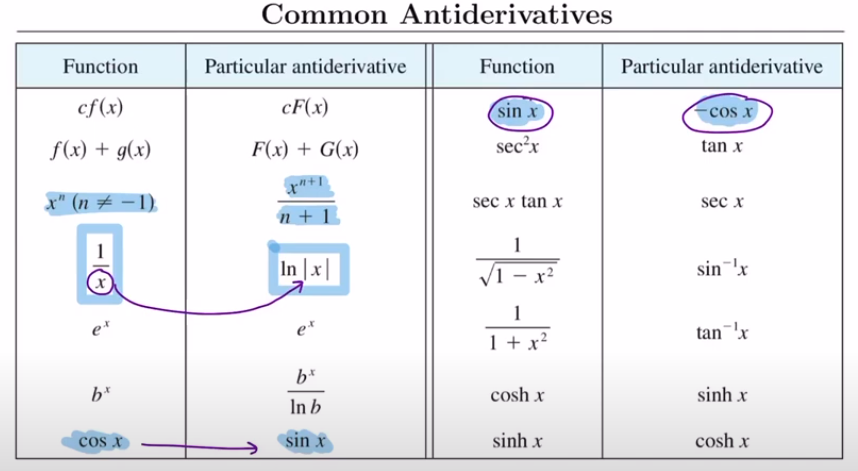
\includegraphics[scale=0.6]{ ../../notes/lectures/chapter4/images/26.png}
      \end{center}


    
\end{document}
